\hl{An oriented diagram $D$ of knot $K$ has two types of crossings, pictured in} \cref{crossing_type}. A diagram coloring, in essence, is an assignment of values from some mathematical object (i.e. $R$-module) to segments of $D$.

\begin{figure}[h]\centering
  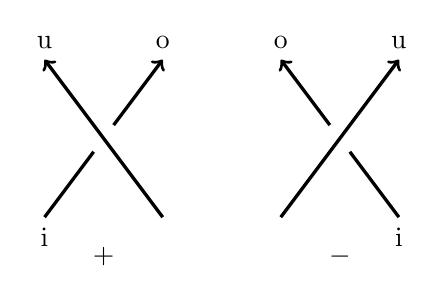
\begin{tikzpicture}
    \draw[very thick, ->] (0,0) node[below] {i} -- (1.5, 2) node[above] {o};
    \fill[white] (0.75, 1) circle (6pt);
    \draw[very thick, ->] (1.5, 0)--(0, 2) node[above] {u};
    \node at (0.75, -0.5) {$+$};

    \draw[very thick, ->] (4.5, 0) node[below] {i} --(3, 2) node[above] {o};
    \fill[white] (3.75, 1) circle (6pt);
    \draw[very thick, ->] (3, 0)--(4.5, 2) node[above] {u};
    \node at (3.75, -0.5) {$-$};
  \end{tikzpicture}
  \caption{Two types of crossing in oriented diagram.\label{crossing_type}}
\end{figure}

\begin{definition}[palette]
  We say that a quadruple {\boldmath$(R, M, \mathcal{C}_\pm)$} is a \buff{palette} if $R$ is a commutative ring with unity, $M$ an $R$-module and $\mathcal{C}_\pm$ are two $R$-modules, corresponding to the two types of crossings (\cref{crossing_type}) such that $\mathcal{C}_\pm\subseteq M^3$.
\end{definition}

We will cumulatively call the two modules $\mathcal{C}_\pm$ the \buff{coloring rule} of palette $(R, M, \mathcal{C}_\pm)$ as they determine whether a coloring is admissible.

\begin{definition}[diagram coloring]
  A \buff{coloring of diagram} $D$ with $s$ segments and $x$ crossings (for knots $s=x$ \cref{ilosc segmentow to ilosc skrzyzowan}) is any element $(m_1,..., m_s)\in M^s$ that assigns elements of $M$ to each arc. 

  We will call a coloring \buff{admissible} if for every crossing $x_j$ of type $\pm$ we have 
  $$\pi_{x_j}(m_1,..., m_s)\in \mathcal{C}_\pm\subseteq\mathcal{C},$$
\hl{where $\pi_{x_j}:M^s\to M^3$ is a projection of module $M^s$ to the $M^3$ factor that corresponds to segments that constitute $x_j$.} 
\end{definition}

Usually, a crossing comprises of exactly three segments. However, as is the case for the first Reidemeister move, a crossing can be comprised of only two segments. Thus, if $x_j$ is such a two-segment crossing, $\im(\pi_{x_j})$ should be isomorphic to $\{(x, y, y)\;:\;x,y\in M\}$.

We can now define two linear homomorphisms
$$\phi_\pm:M^3\to M^3/\mathcal{C}_\pm=N_\pm$$
that take in as arguments the arcs constituting a crossing. Assuming that $M^3/\mathcal{C}_\pm\cong M$ (reasoning behind this assumption will be given in \cref{section 3.2}), we will take 
\begin{align}
  \phi_+(u,i,o)=au+bi+co \label{phi equations1} \\ 
  \phi_-(u,i,o)=\alpha u+\beta i+\gamma o \label{phi equations2}
\end{align}
for $u$, $i$, $o$ understood like in \cref{crossing_type} and with coefficients being homomorphisms $M\to M$.

\begin{lemma}\label{proposition male kernel kolorowania}
  A coloring $(m_1,..., m_s)\in M^s$ is a admissible $\iff$ for each crossing $x_j$ of type $\pm$ 
  $$\phi_\pm(\pi_{x_j}(m_1,...,m_s))=0.$$
\end{lemma}

\begin{proof}
  Stems from the fact that $\mathcal{C}_\pm=\ker\phi_\pm$.
\end{proof}

